\documentclass{standalone}
\usepackage{tikz}

\begin{document}
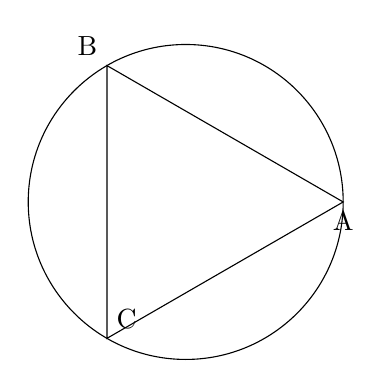
\begin{tikzpicture}
    % Draw the circle
    \draw (0,0) circle (2cm);
    
    % Define the points of the equilateral triangle
    \coordinate (A) at (0:2cm);
    \coordinate (B) at (120:2cm);
    \coordinate (C) at (240:2cm);
    
    % Draw the equilateral triangle
    \draw (A) -- (B) -- (C) -- cycle;
    
    % Optionally, label the vertices
    \node at (A) [below] {A};
    \node at (B) [above left] {B};
    \node at (C) [above right] {C};
\end{tikzpicture}
\end{document}